\section{Studies of signal and background separation using Mann-Whitney U test}
In this section, we study different jet substructure variables and compare their ability to separate the signal and the background for different detector sizes using Mann-Whitney U test.\\

In the Mann Whitney U test by definition, if U value is closed to 0.5, it means two distributions have similar compositions, and we can't distinguish them very well. On the other hand, if U value of two distributions are closed to 0, it means both distributions' compositions are much different from each other. For another point of view, if U value is closed to 0.5, separation power of certain variable is bad, instead, if U value is closed to 0, separation power is great.\\

Figure 6 shows the representative samples of the distributions about the U value for $\tau_{21}$,$\tau_{32}$ in different detector sizes. In $\tau_{21}$, separation power is improved when detector size is smaller, but in $\tau_{32}$, the smallest detector sizes isn't the best one to separate signal and background.\\

In Figure 7, it shows the summary plots about the clustering in Mann Whitney U test in three different variables. In $\tau_{21}$, 5TeV has better separation power when detector sizes are getting smaller, but when energy higher than that, there is no improvement in smaller detector. In $\tau_{32}$, the case is similar to  $\tau_{21}$. Even worse, at some collision energies, bigger detector sizes have better separation power than smaller detector sizes. In $c_2^{(1)}$, all separation power aren't improved by detector sizes.  In summary, $c_2^{(1)}$ is the best parameter, because all values are smaller than other parameters compare with the same energy collision, and its separation power don't have the significant improvement in higher energy collision.

In Figure 8 , it shows the summary plots about the rawhit cut at 0.5GeV in Mann Whitney U test in three different variables. In $\tau_{21}$, 5TeV and 10TeV have better separation power in smaller separation power, but when energy higher than that, it won't improve.  In $\tau_{32}$, all separation power aren't improved by detector sizes. In $c_2^{(1)}$, we can see in 5,10,20TeV, separation power will be improved slightly, but at 40TeV, it won't improve. In summary, $c_2^{(1)}$ has the highest power separation at highest collision energy.

\label{sec:Mann Whitney U test}


\begin{figure}
\begin{center}
   \subfigure[20$\times$20(cm$\times$cm)] {
   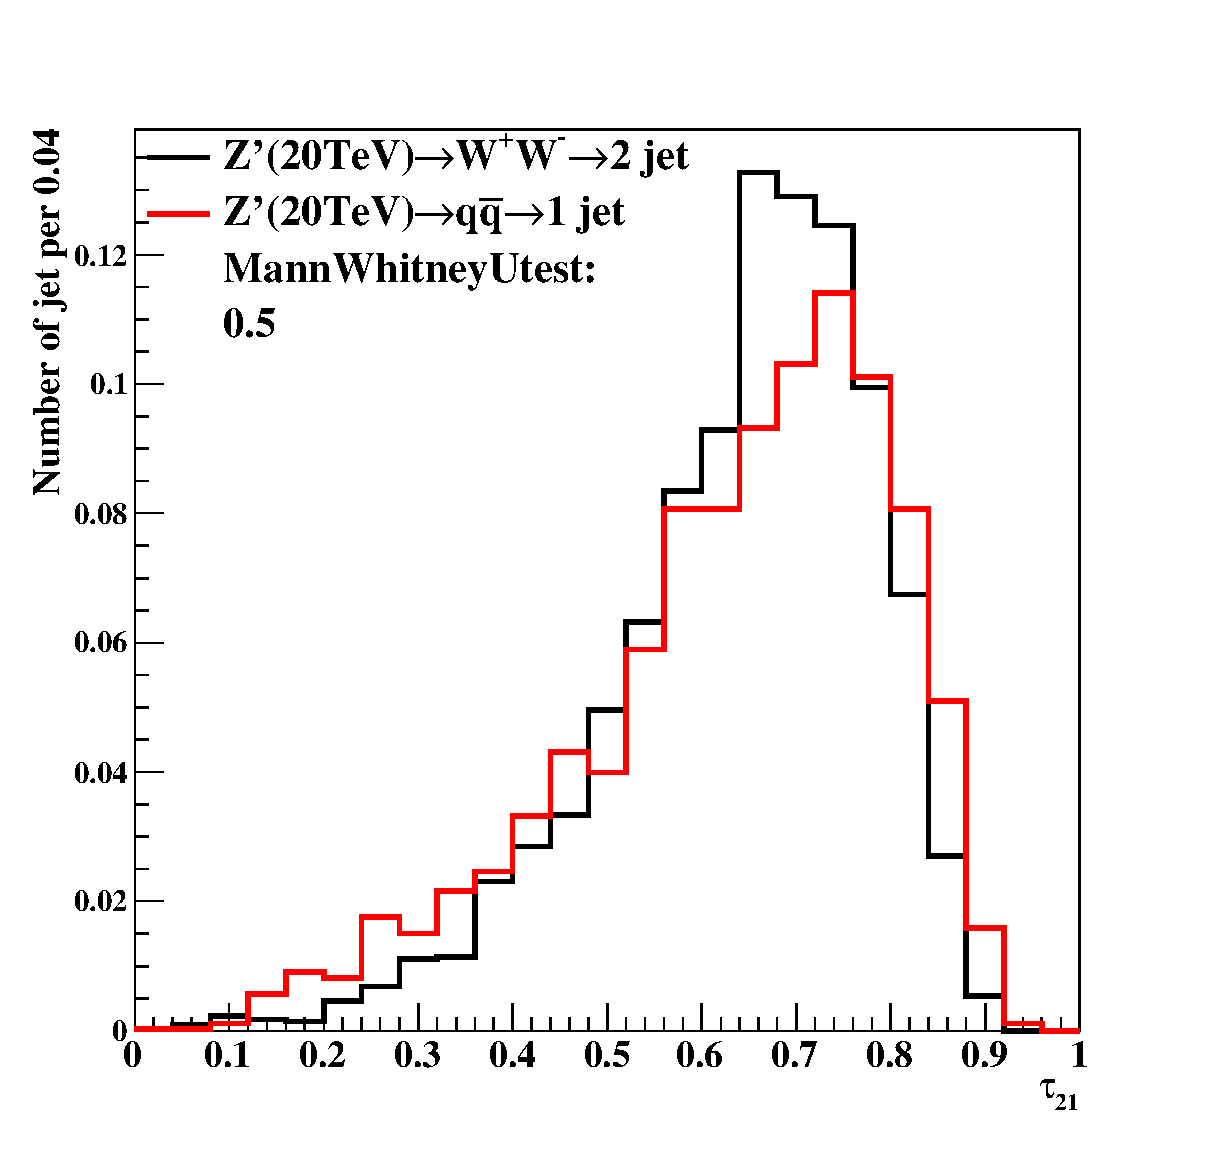
\includegraphics[width=0.43\textwidth]{figs/r009_tau21b1_20tev_04_U.eps}\hfill
   }
   \subfigure[20$\times$20(cm$\times$cm)] {
   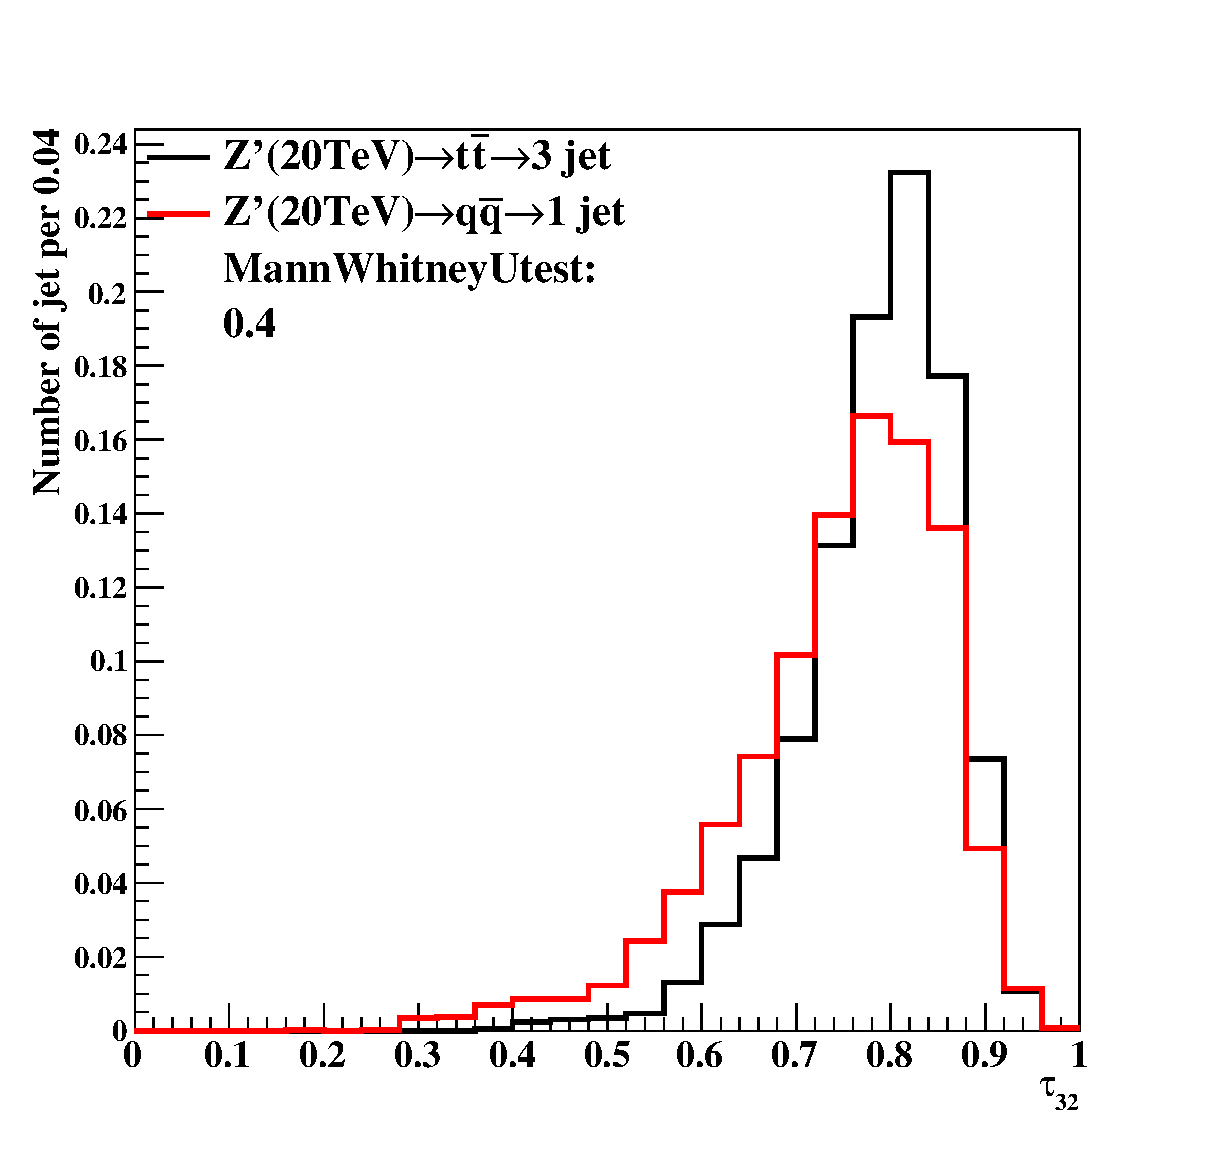
\includegraphics[width=0.43\textwidth]{figs/r009_tau32b1_20tev_04_U.eps}
   }
   \subfigure[5$\times$5(cm$\times$cm)] {
   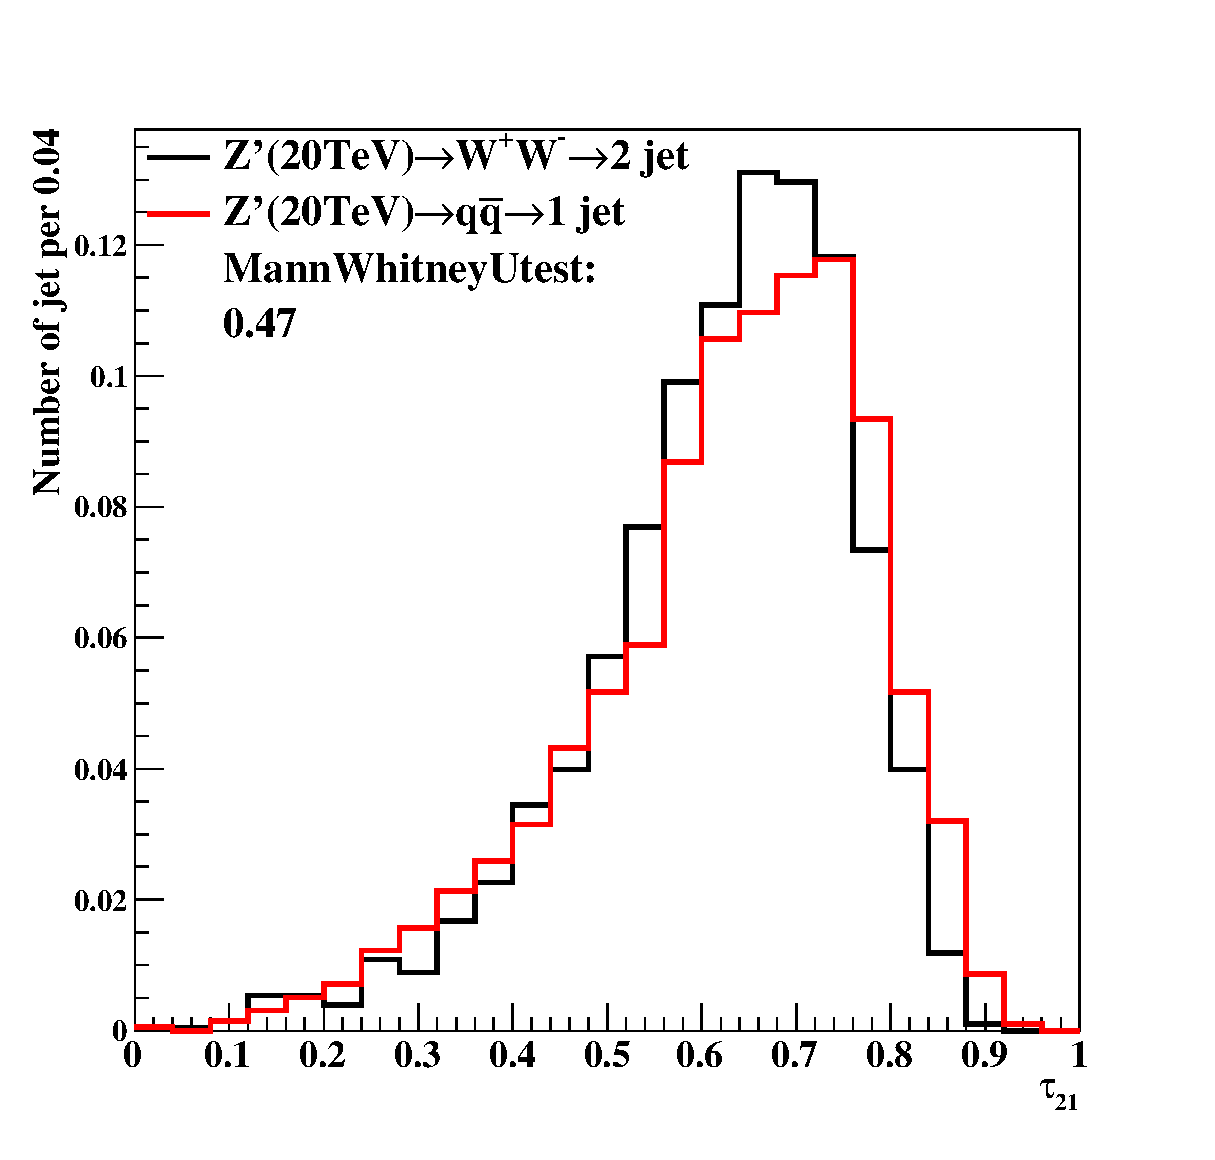
\includegraphics[width=0.43\textwidth]{figs/r010_tau21b1_20tev_04_U.eps}
   }
   \subfigure[5$\times$5(cm$\times$cm)] {
   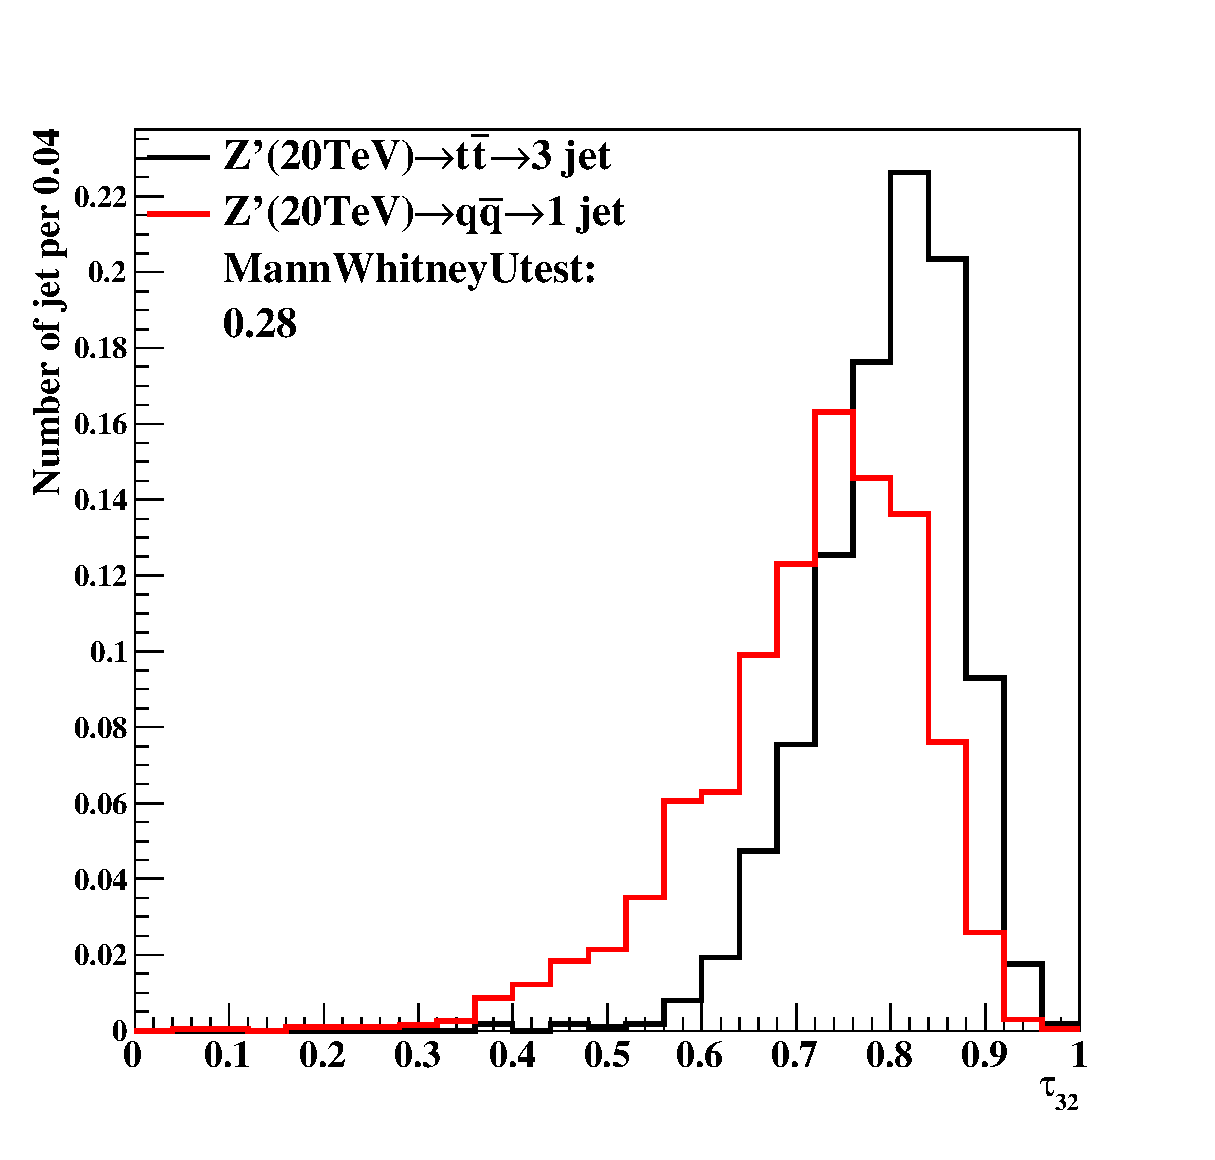
\includegraphics[width=0.43\textwidth]{figs/r010_tau32b1_20tev_04_U.eps}
   }
   \subfigure[1$\times$1(cm$\times$cm)] {
   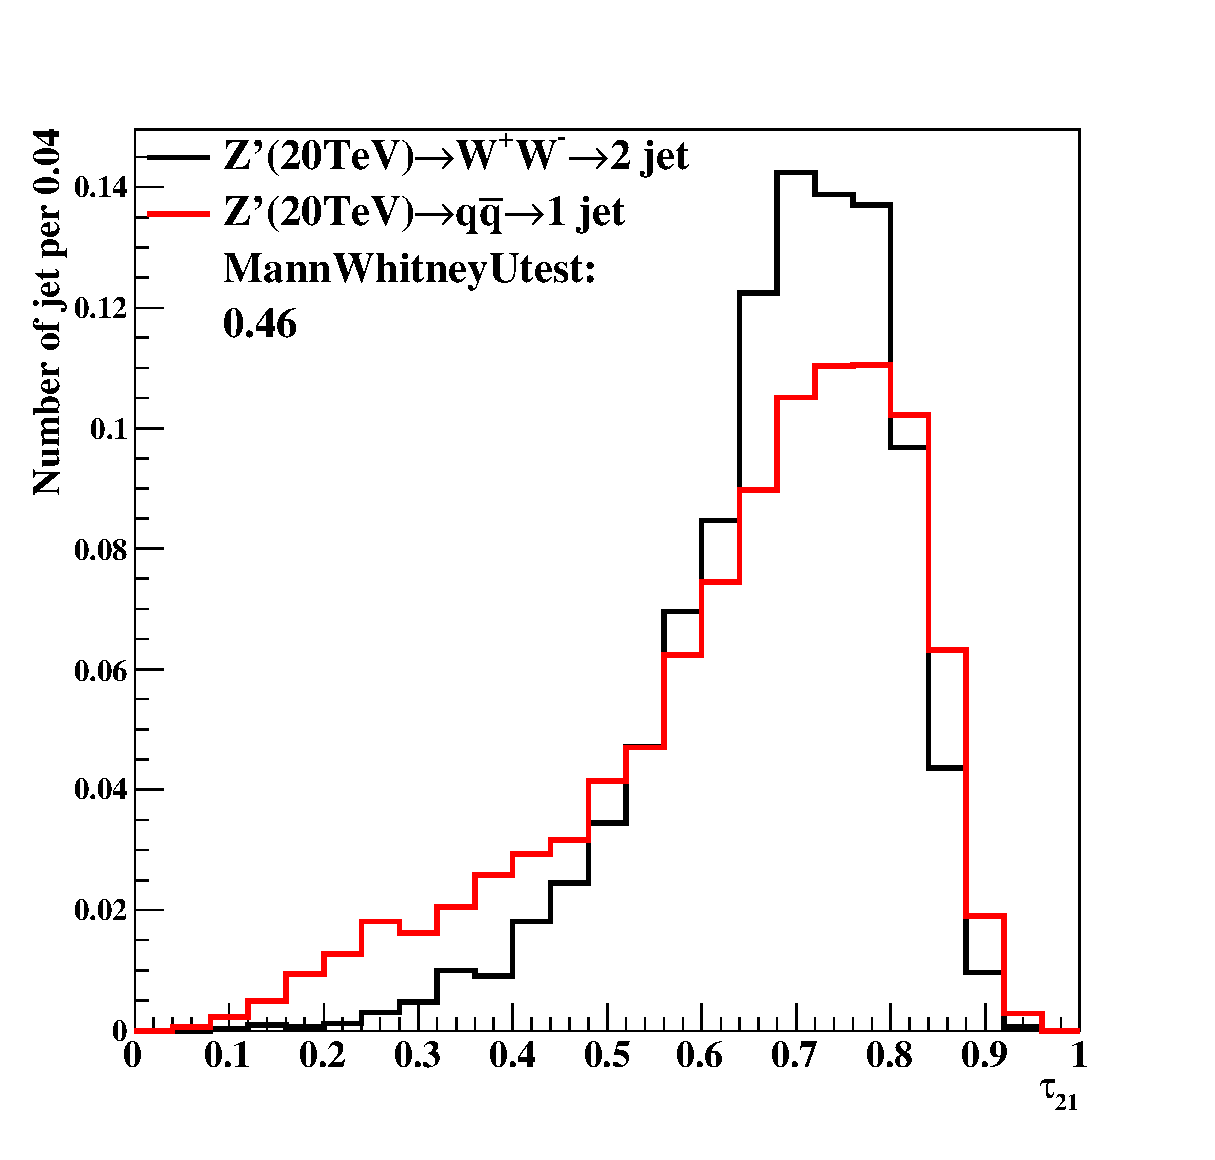
\includegraphics[width=0.43\textwidth]{figs/r012_tau21b1_20tev_04_U.eps}
   }
   \subfigure[1$\times$1(cm$\times$cm)] {
   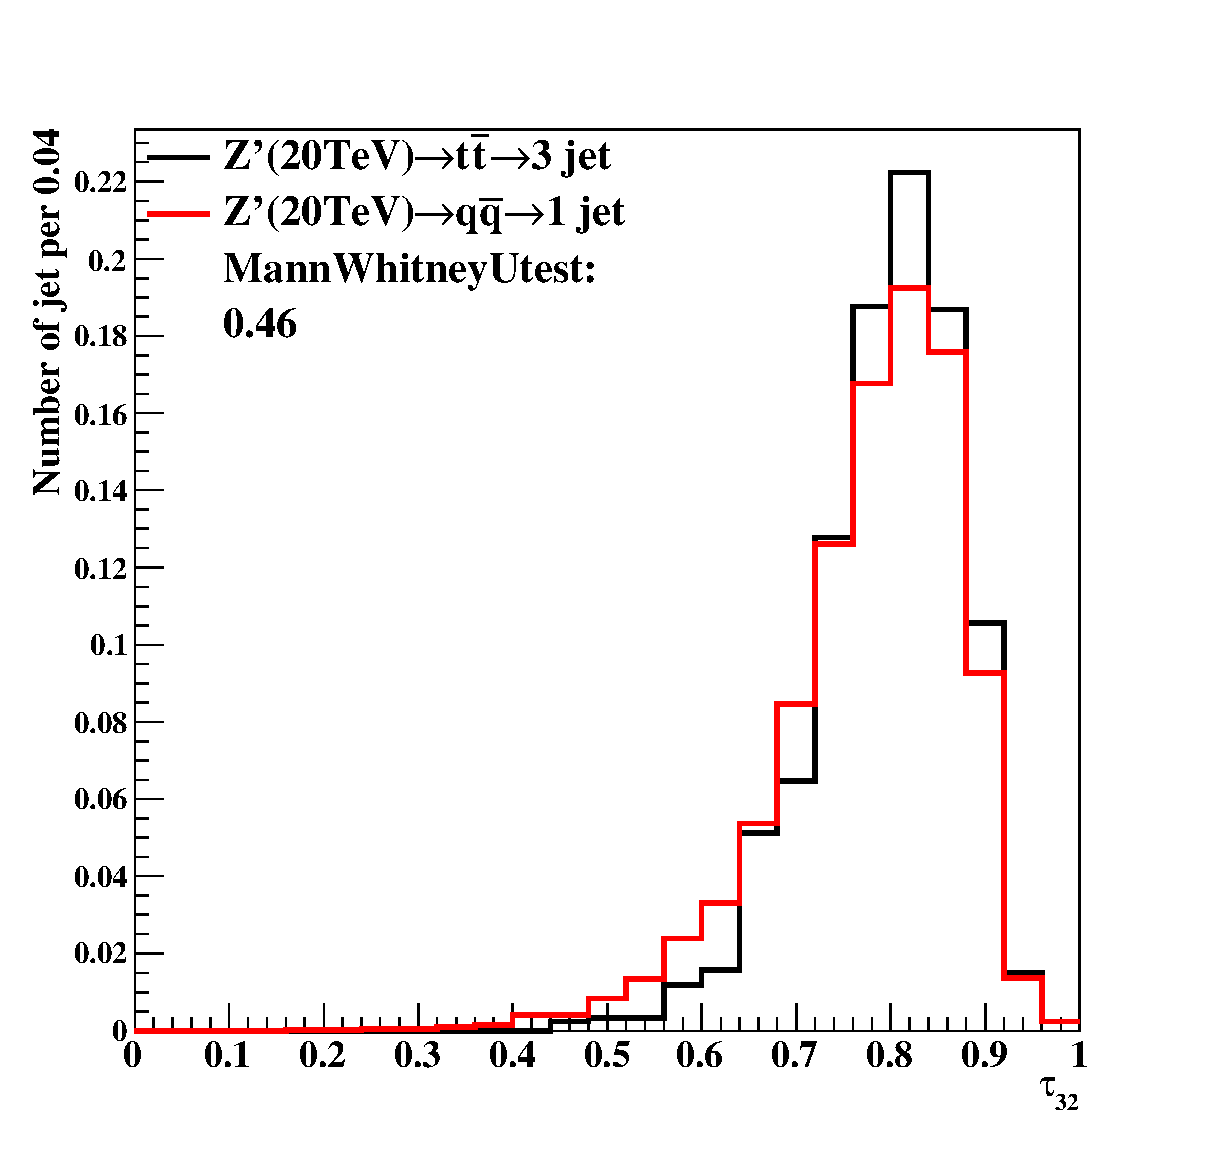
\includegraphics[width=0.43\textwidth]{figs/r012_tau32b1_20tev_04_U.eps}
   }

\end{center}
\caption{Distributions and U value in 20TeV energy collision for $\tau_{21}$,$\tau_{32}$ in different detector sizes.}
\label{fig:cluster_tau21_tau32}
\end{figure}


\begin{figure}
\begin{center}
   \subfigure[$\tau_{21}$] {
   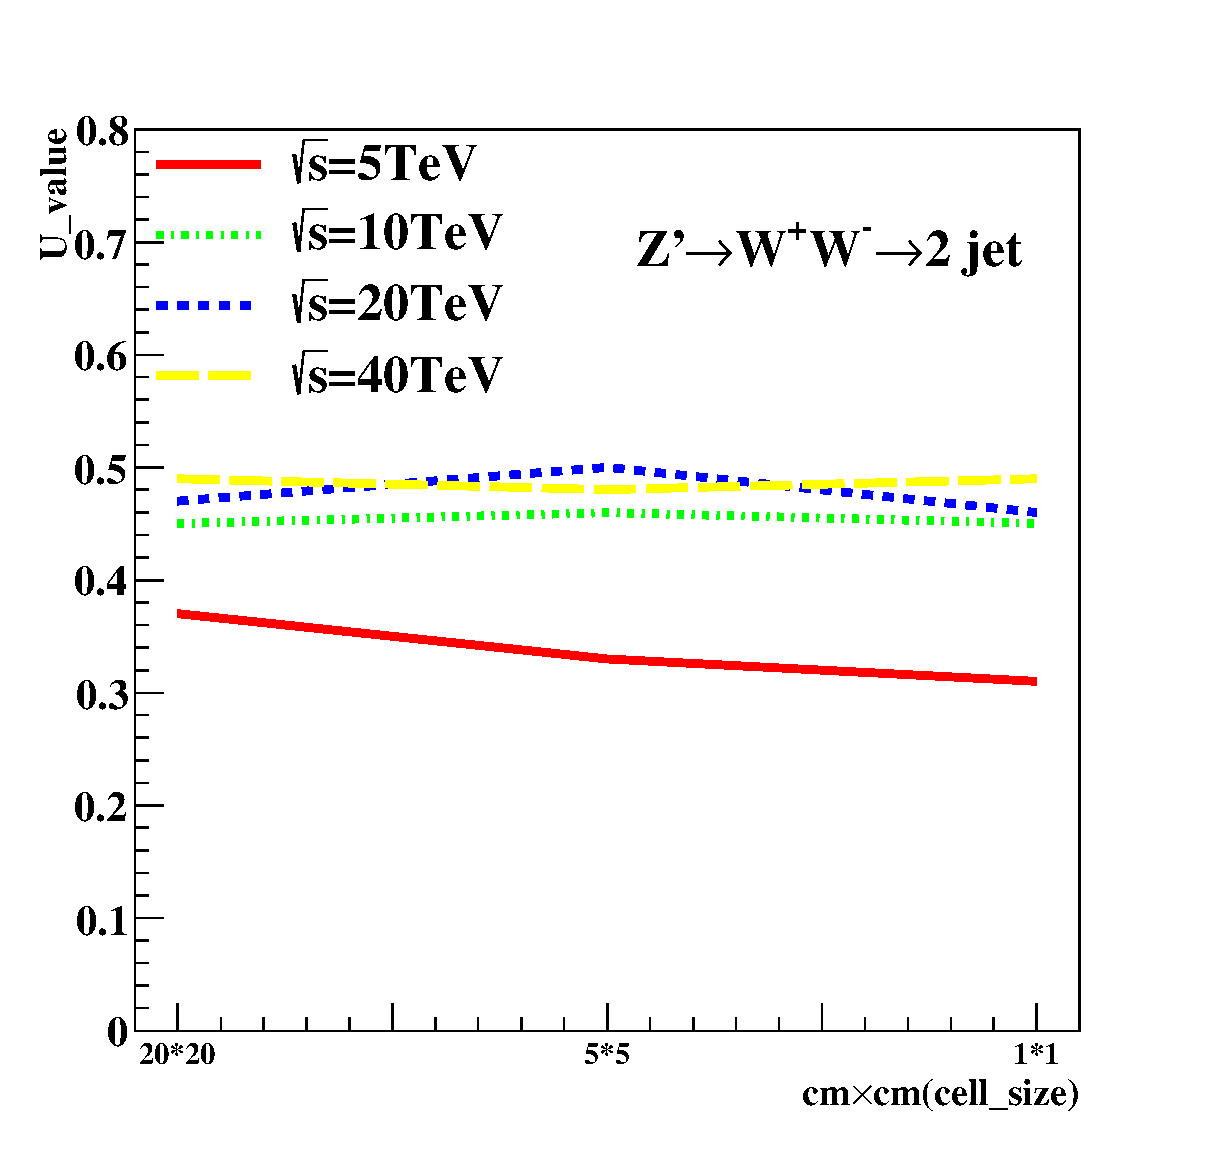
\includegraphics[width=0.43\textwidth]{figs/cluster_tau21_summary_U.eps}\hfill
   }
   \subfigure[$\tau_{32}$] {
   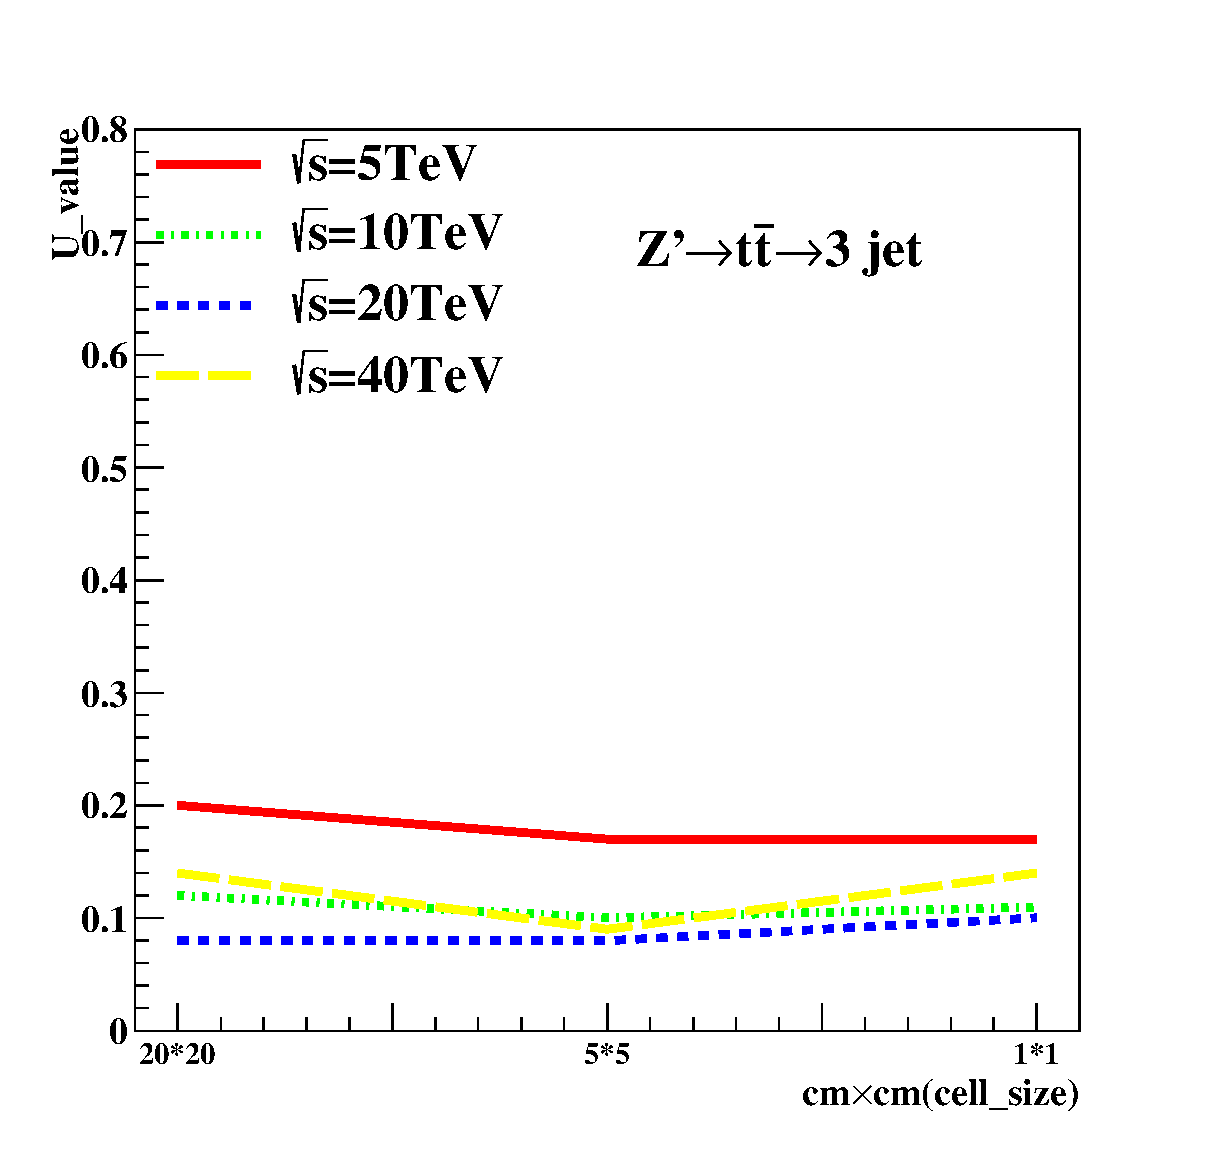
\includegraphics[width=0.43\textwidth]{figs/cluster_tau32_summary_U.eps}
   }
   \subfigure[$c_2^{(1)}$] {
   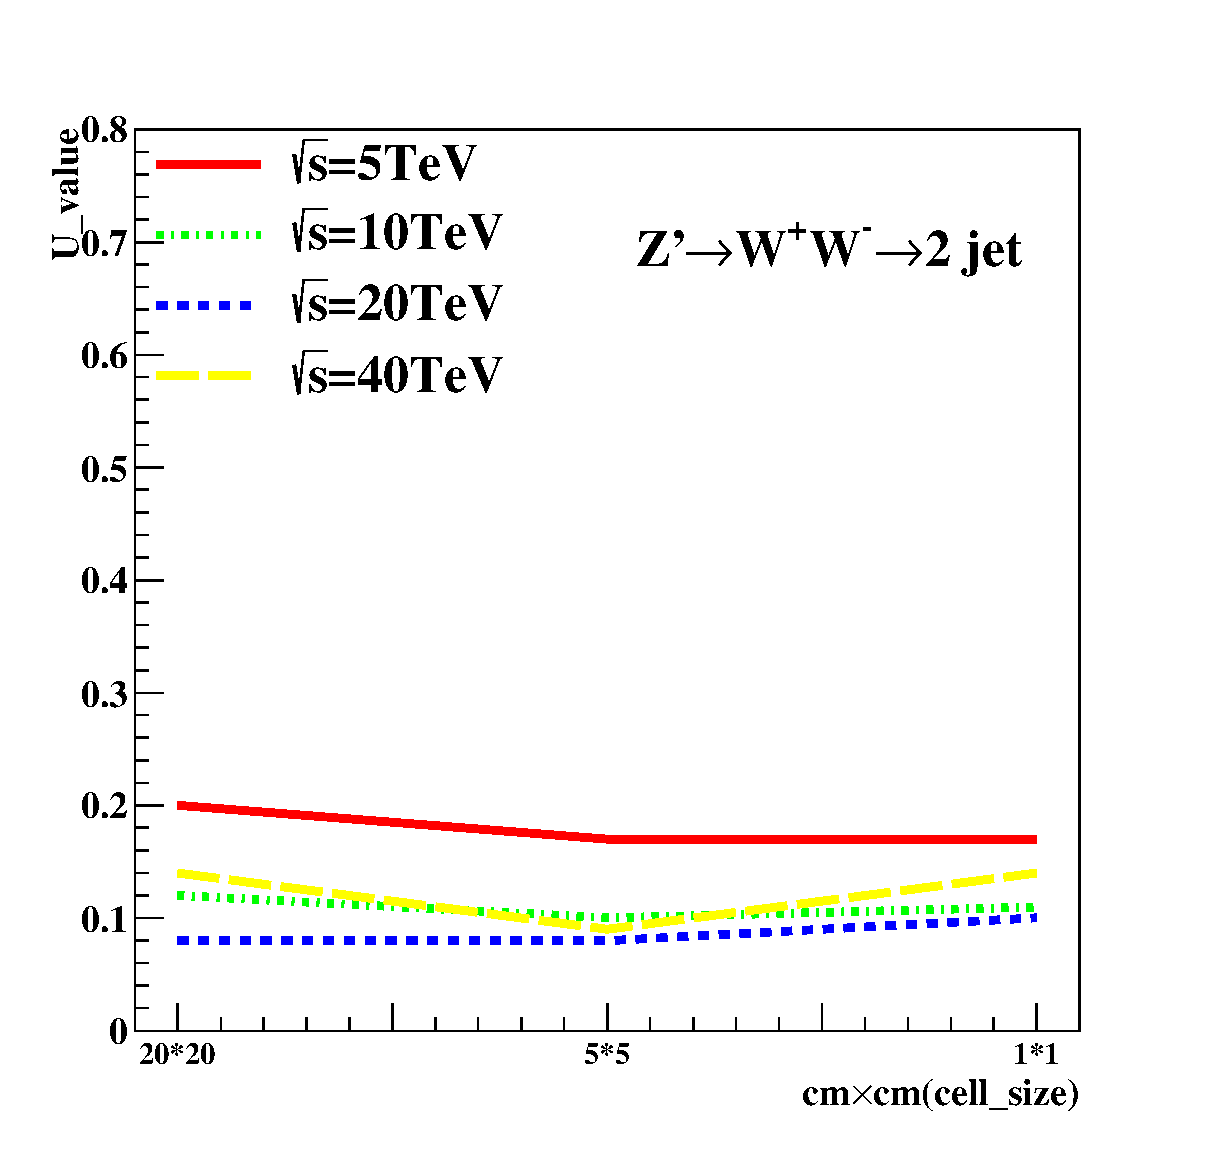
\includegraphics[width=0.43\textwidth]{figs/cluster_c2b1_summary_U.eps}
   }
\end{center}
\caption{Different U value of collision energies correspond to different different detector sizes in cluster. The energies of collision at 5,10, 20, 40TeV are shown in all pictures.}
\label{fig:cluster_U_summary}
\end{figure}


\begin{figure}
\begin{center}
   \subfigure[$\tau_{21}$] {
   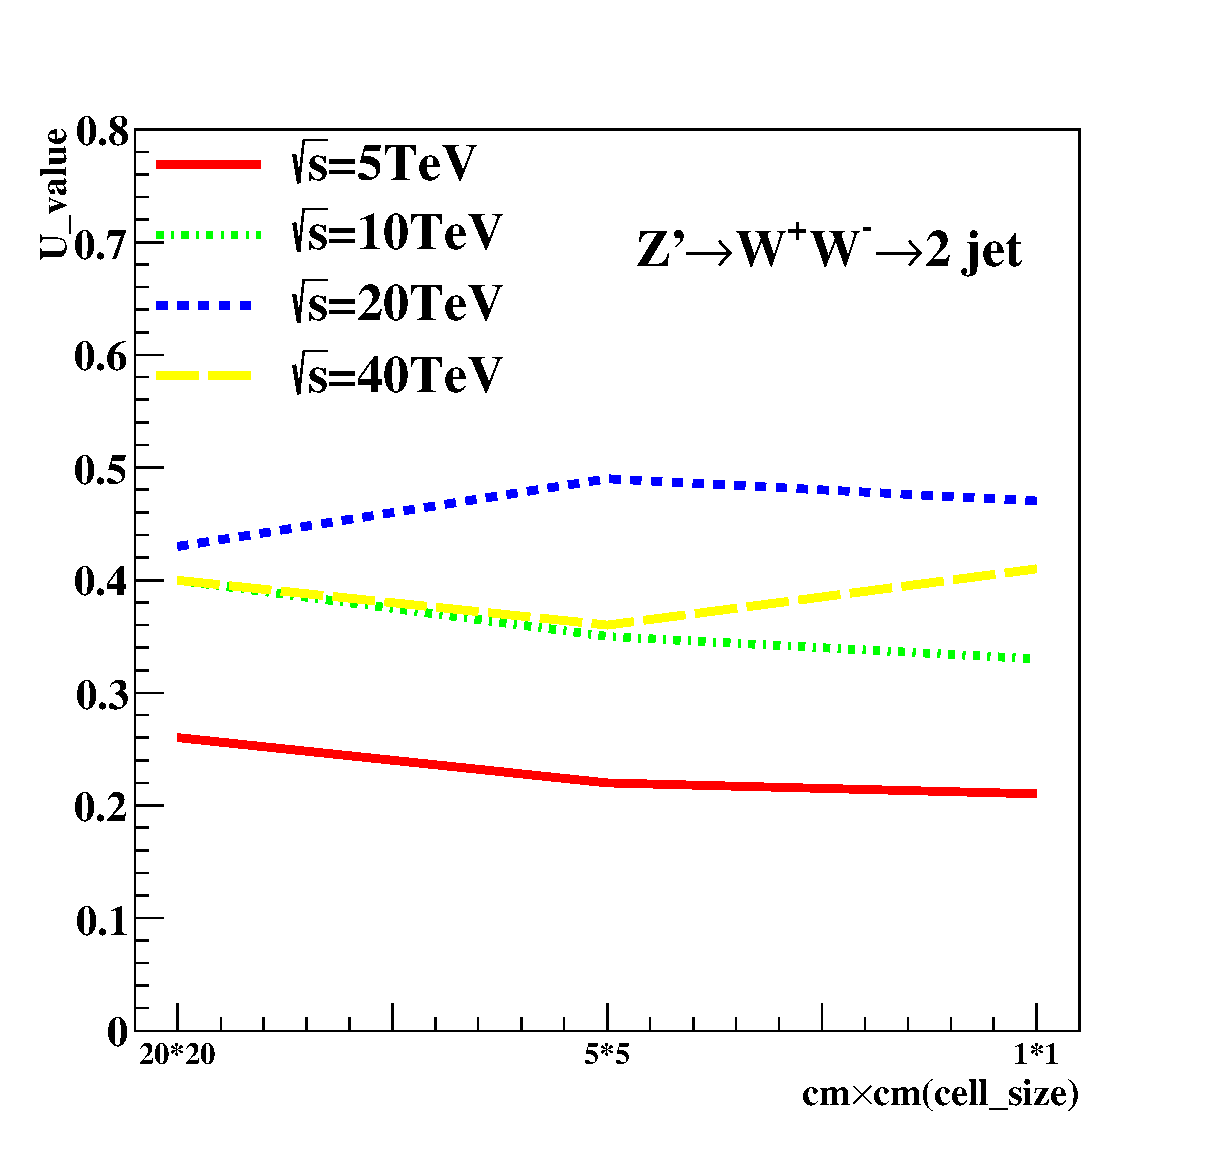
\includegraphics[width=0.43\textwidth]{figs/raw_tau21_summary_U.eps}\hfill
   }
   \subfigure[$\tau_{32}$] {
   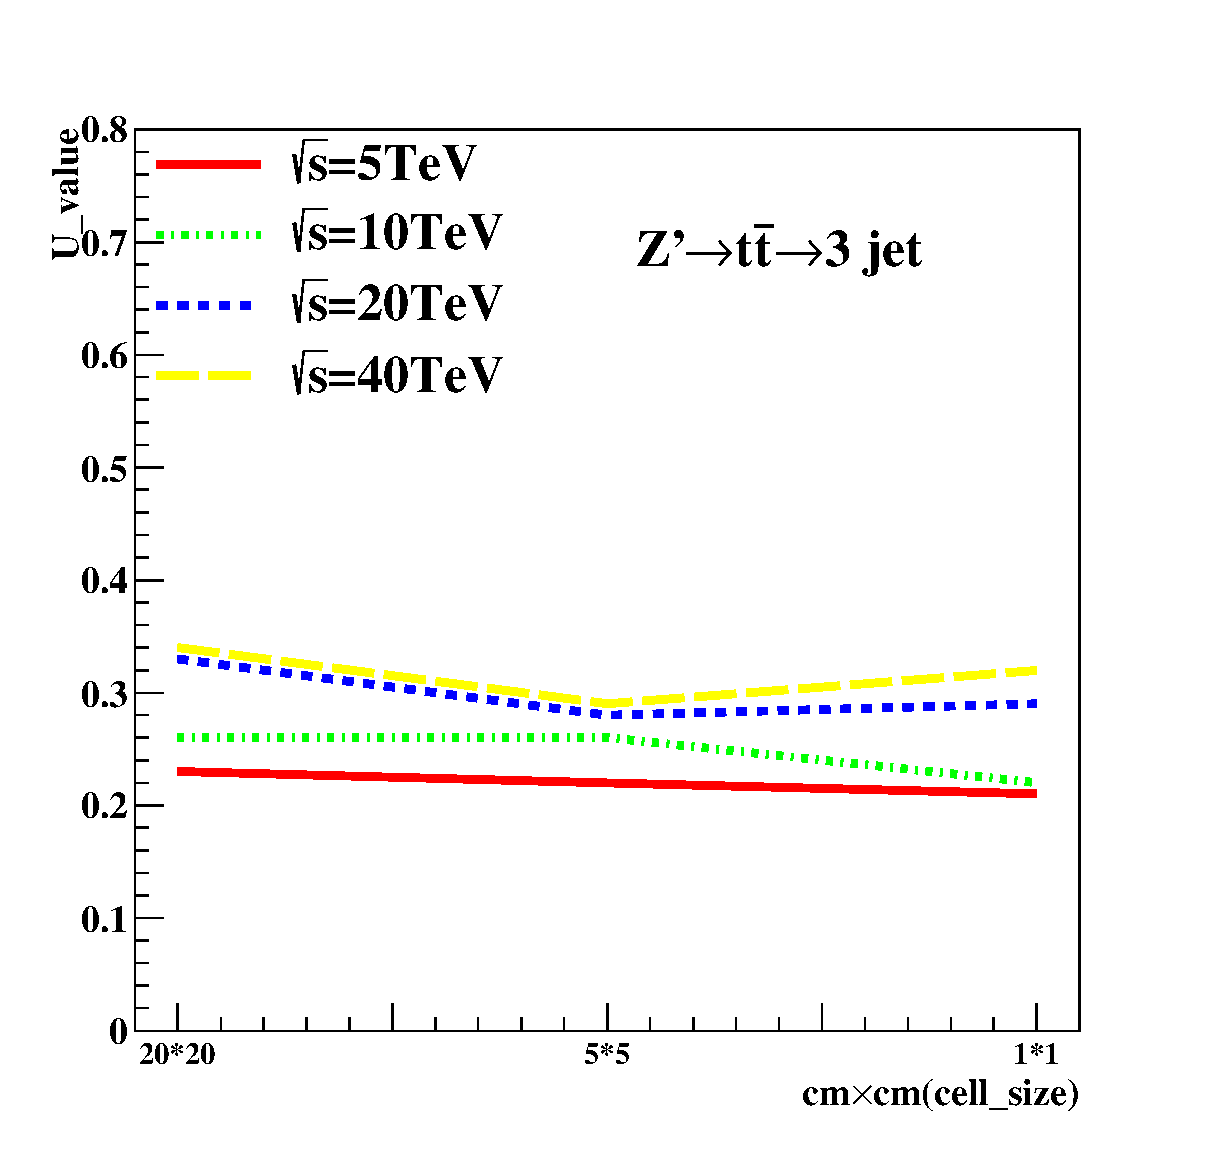
\includegraphics[width=0.43\textwidth]{figs/raw_tau32_summary_U.eps}
   }
   \subfigure[$c_2^{(1)}$] {
   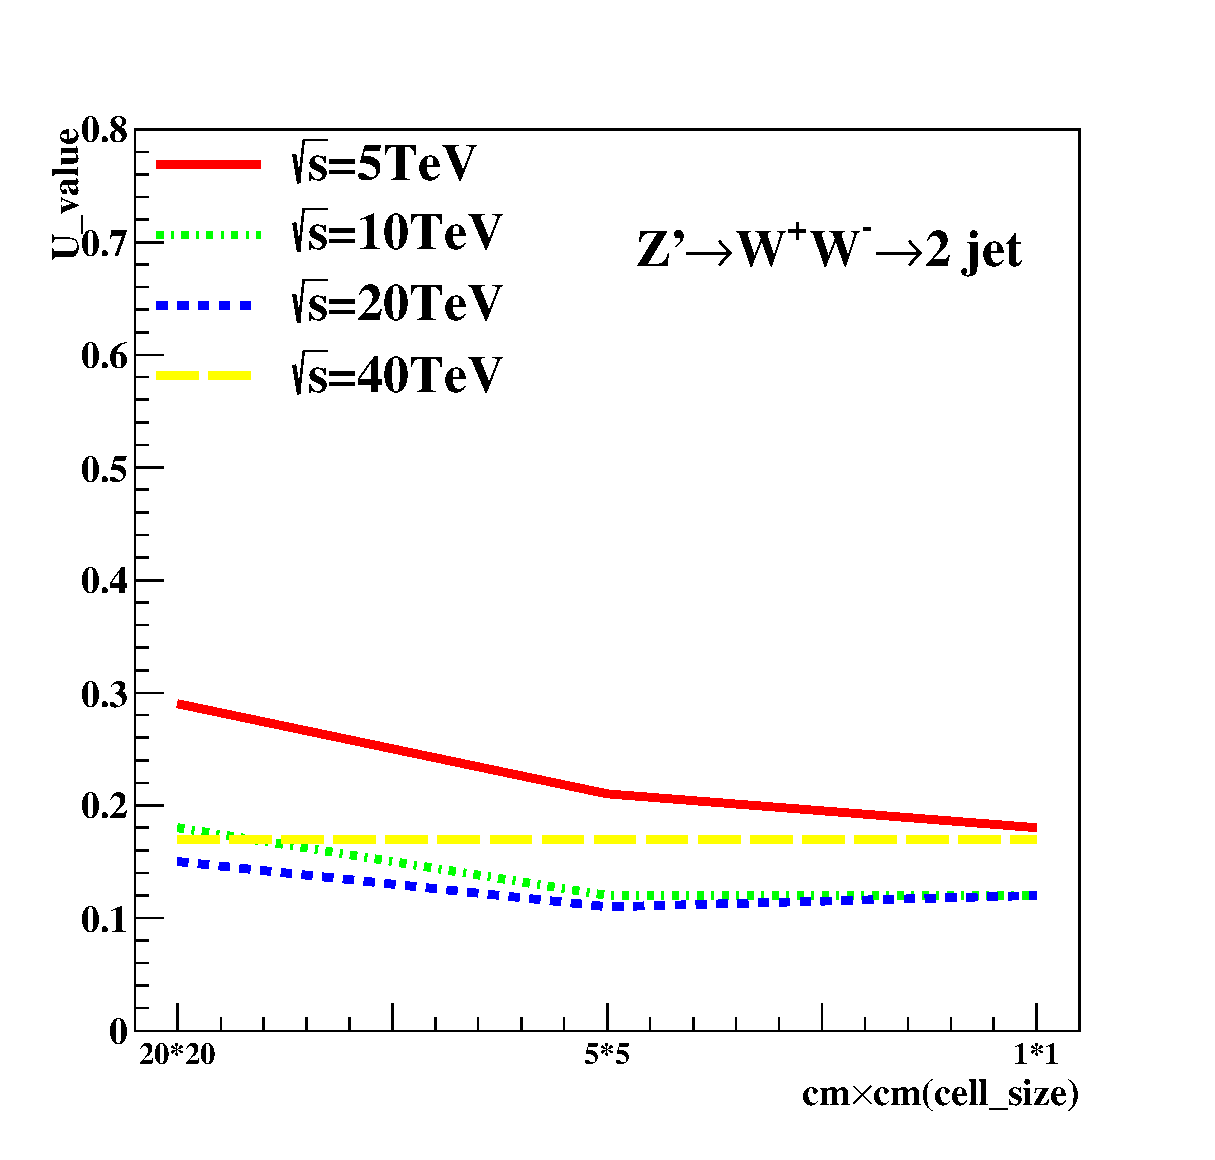
\includegraphics[width=0.43\textwidth]{figs/raw_c2b1_summary_U.eps}
   }
\end{center}
\caption{Different U value of collision energies correspond to different different detector sizes in rawhit cut at 0.5GeV. The energies of collision at 5,10, 20, 40TeV are shown in all pictures.}
\label{fig:raw_U_summary}
\end{figure}

